\subsection{Mandatory Performance (\textit{JJ, MK})}
\label{mand}
The AIAA RFP \cite{RFP} requires this short range aircraft to have a range of 3,500 NM with the ability to carry a capacity of 400 passengers in a dual class configuration. The aircraft must also have enough reserves to fly to an alternate airport 200 NM from the destination airport, hold for 30 minutes at the alternate airport, and contain 5\% contingency fuel, which is defined as 5\% of non-reserve block fuel. Furthermore, both takeoff and landing distances are restrained to 9,000 ft or less off asphalt or concrete runways at International Standard Atmosphere (ISA) +15 degrees Celsius conditions. Finally, the maximum approach speed the aircraft can have is 145 knots calibrated airspeed (KCAS) at the end of the design mission. 

% \subsection{Predicted Performance (\textit{MK})}
% First-cut analysis was performed using an estimated empty weight as well as a fuel weight calculated by using a thrust-specific fuel consumption (TSFC) average of contemporary large turbofan engines, such as what would be found on an aircraft of this size.  This data was then input into a time-step integration spreadsheet to converge on a first design for a bounded range for cruise. For the duration of cruise, the aircraft will begin cruising at an altitude of FL370, where it will perform two step climbs of 3000 ft each and end at a cruising altitude of FL430. Before and after cruise, the aircraft will follow the mission profile as stated in Section \ref{section: Conops} in Figure \ref{fig:missionprof}.

% In the future, the flight envelope as well as fuel estimation of each segment in the mission profile will be performed. Additionally, the time-step integration of cruise will be refined and the time-step integration process will be implemented for the climb, descend, and loiter segments of the mission. Further analysis will performed on determining the drag of each mission segment as well as regulating that the design stays within the requirements set forth by the RFP \cite{RFP}. obsolete now

\subsection{Determination of Cruising Altitude (\textit{MK})}
To determine a valid cruising altitude, a trade study was performed on the two-class capacity of similiar aircraft that either are currently in service or were in the past. This will facilitate the decision of which altitude will be best to cruise at for SAM Mk 1. Figure \ref{cruxalt} shows four aircraft and their respective cruising altitudes and two-class passenger capacity\cite{butterworth}.

\begin{table}[!h]
    \centering
        \caption{Cruise Altitude Comparison of Similar Capacity Aircraft}
    \begin{tabular}{|c||c|c|c|c|}\toprule
         & \textbf{B747-200} & \textbf{B777-200} & \textbf{A340-600} & \textbf{IL96-M}\\ \hline \hline
         \textbf{Manufacturer} & Boeing & Boeing & Airbus & Ilyushin \\ \hline
         \textbf{Cruise Altitude [ft]} &  35,000 & 39,000 & 41,000 & 30,000 \\ \hline
         \textbf{2-Class Capacity} & 442 & 375 & 440 & 335\\ \bottomrule
    \end{tabular}
    \label{cruxalt}
\end{table}

From the trade study, it can be seen that all the aircraft listed range in cruising altitudes from 35,000 ft to 41,000 ft. The next step was taken the average of each aircraft's cruising altitude and passenger capacity. The average cruising altitude between the aircraft is 36,500 ft, while the average passenger capacity is 398 passengers. From these averages, similar capacity aircraft tend to cruise at an altitude just above the tropopause. Thus, from analysis, Team Toucan has decided to design SAM Mk. I to cruise at an altitude of 37,000 ft.

\subsection{Determination of Cruise Speed}
\label{crusspeed}
\subsubsection{Trade Study of Commercial Aircraft Cruise Speeds (JJ)}
A trade study of common turbine-powered commercial aircraft ranging in size and age from both Boeing and Airbus was performed on the basis of determining their respective cruise speed and maximum fuel range (as reported by manufacturer).  All data used in this trade study came from one source:  \cite{butterworth}, with the cruise speed converted from velocity to Mach number at the specified cruise altitude respective to each plane. 

\begin{table}[!h]
    \centering
        \caption{Comparison of Cruise Speed for Turbine-Powered Aircraft}
    \begin{tabular}{|p{1.1in}||c|c|c|c|c|c|c|}\toprule
         & \textbf{B747-400} & \textbf{B757-200} & \textbf{B767-400} & \textbf{B777-200} & \textbf{A320-200} & \textbf{A330-300} & \textbf{A340-600} \\\hline \hline
         \textbf{Manufacturer} & Boeing & Boeing & Boeing & Boeing & Airbus & Airbus & Airbus\\ \hline
         \textbf{Cruise Mach} & 0.85 & 0.80 & 0.80 & 0.75 & 0.74 & 0.76 & 0.82\\ \hline
         \textbf{Max. Range [NM]} & 7260 & 4488 & 5625 & 4820 & 3672 & 7046 & 7800 \\ \bottomrule
    \end{tabular}
    \label{tab:cruisecomp}
\end{table}

\newpage
This information leads to a mean cruise speed (of these selected planes) equal to Mach 0.788.  This study was performed to augment the analytical determination, \ref{cruisespeed}, as factors such as time of flight and airline (operator) preference also play a role in determining a desirable cruise speed.

\subsubsection{Analytical Determination of Cruise Speed (\textit{MK})} \label{cruisespeed}
It is established that best aerodynamic performance during steady, level flight (cruise) corresponds to the same maximum range speed as the occurrence of $(\frac{C_{L}^{1/2}}{C_{D}})_{max}$, which corresponds to the minimum power required. This can be found analytically by plotting total drag on a thrust required versus velocity chart. Then, the local minimum corresponds to $(\frac{C_{L}^{1/2}}{C_{D}})_{max}$, which then indicates the optimal Mach number. Figure \ref{optimach} visually demonstrates this theory, and shows the optimal Mach number to be 0.996 at a $(\frac{C_{L}^{1/2}}{C_{D}})_{max}$ of 23.9. 

Now, comparing the analytical method to the trade study, the values vary by quite a bit. However, the Mach number determined through the analytical method is much higher than what aircraft of this type and size usually have. This could be due to the plot underestimating the amount of drag. Thus, for the remainder of the project, Team Toucans decided to choose a Mach number to be slightly less than the trade study Mach number, with a greater weight applied towards the Mach number determined from trade study. The final cruise Mach number was chosen to be Mach 0.775.

\begin{figure}[H]
    \centering
    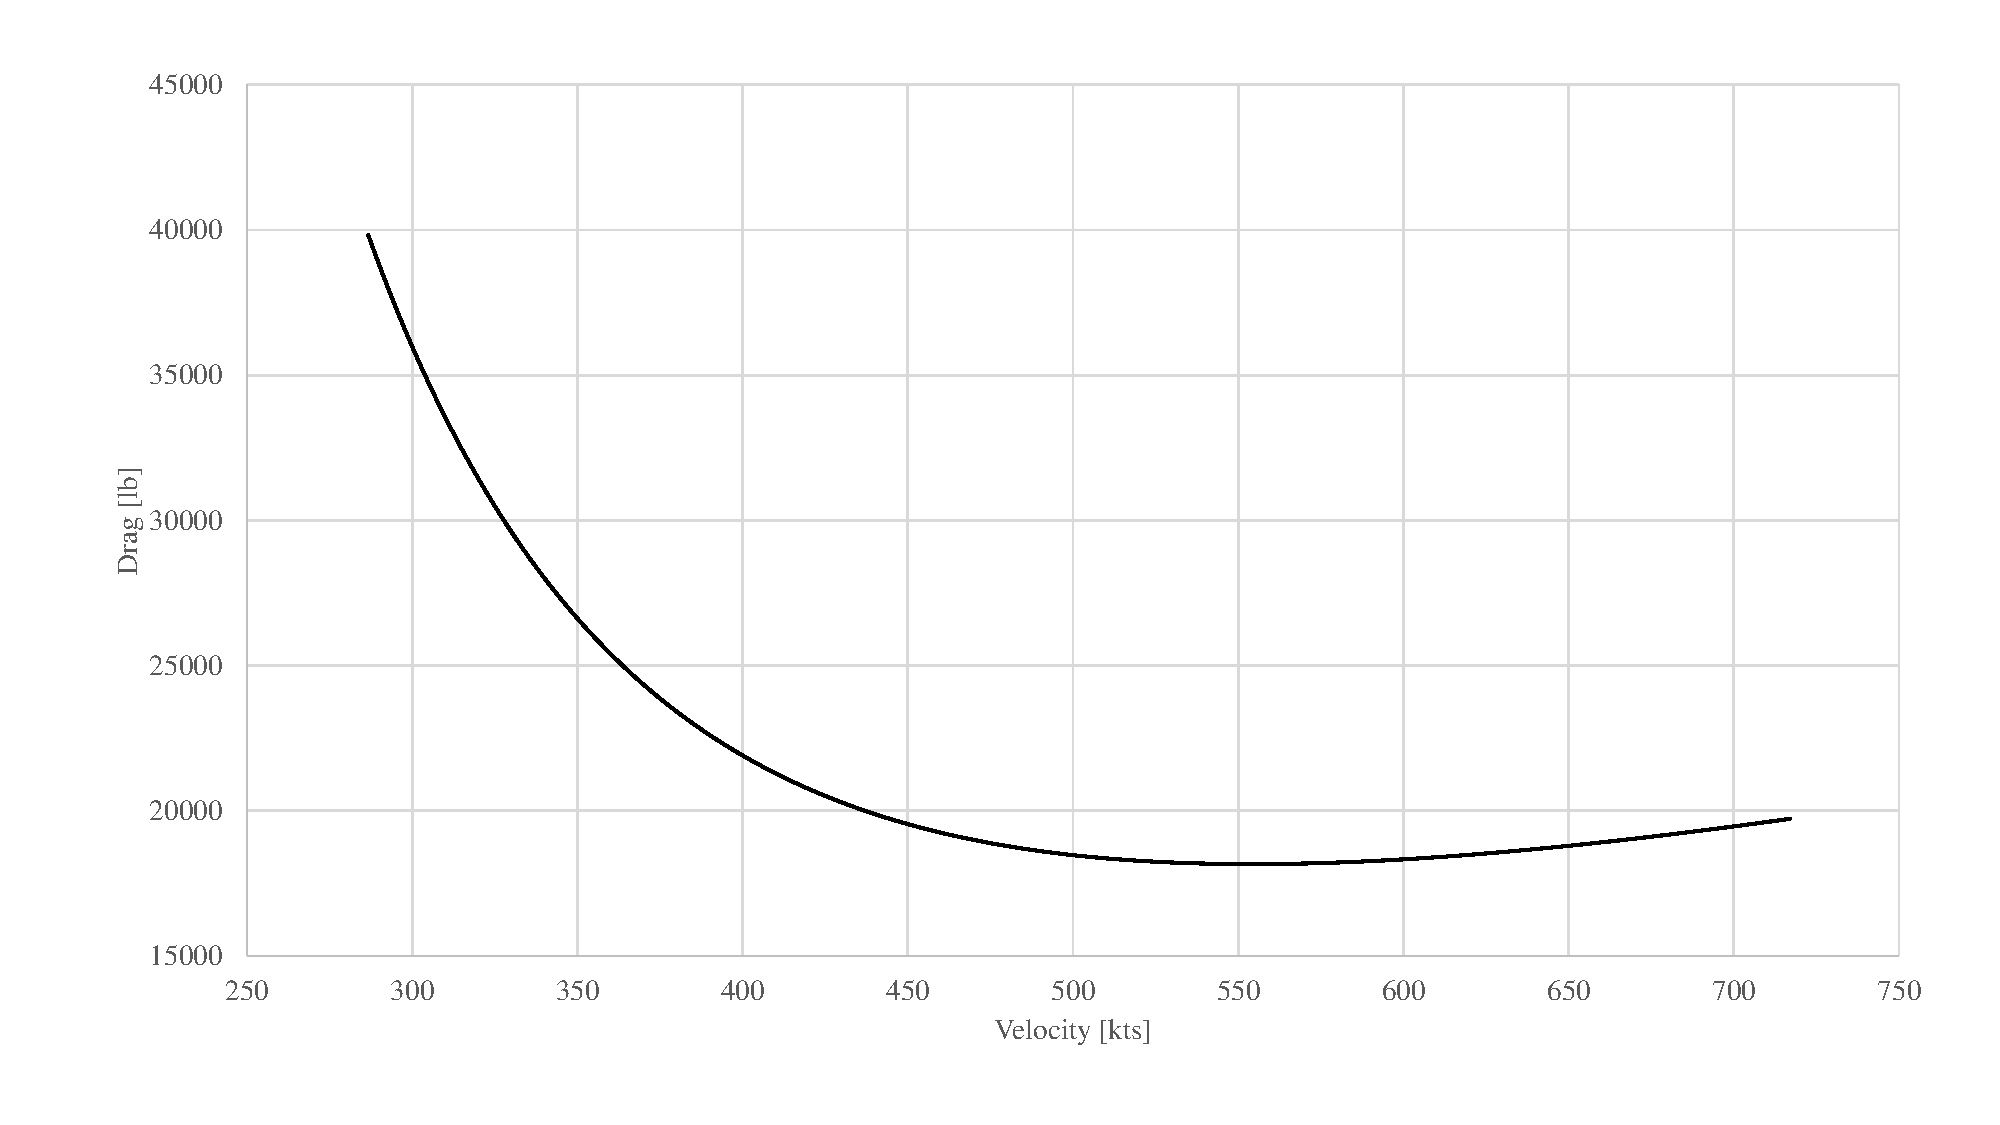
\includegraphics[width=1.0\textwidth]{Photos/Optimal_Mach.pdf}
    \caption{Optimal Mach Number at \boldmath{$(\frac{C_{L}^{1/2}}{C_{D}})_{max}$}}
    \label{optimach}
 \end{figure}

\subsection{Takeoff and Landing Analysis (\textit{MK})}
\qquad
When analyzing takeoff and landing distances, Team Toucan used the methods described in Raymer \cite{raymer} Chapter 17 and accounted for multiple runway conditions. Specifically, the ground roll, rotation, transition and climb distances for take-off along with the approach, flare and ground distances for landing are shown in Table \ref{tab:TO} and Table \ref{tab:land}, respectively. The takeoff distances were calculated assuming OEI, which follows the certification CFR Part 25.107 \cite{cfr}.

\begin{table}[!h]
    \centering
    \caption{Takeoff Distance - Each Segment}
    \begin{tabular}{|>{\centering}p{1.1in}|>{\centering}p{.3in}|>{\centering}p{1.0in}|>{\centering}p{.75in}|>{\centering}p{.83in}|>{\centering}p{.6in}|>{\centering\arraybackslash}p{.6in}|}\toprule 
    \textbf{Runway Condition} & \boldmath{$\mu$} \textbf{\cite{raymer}} & \textbf{Ground Roll [ft]} & \textbf{Rotation [ft]} & \textbf{Transition [ft]} & \textbf{Climb [ft]} & \textbf{TOFL [ft]} \\ \hline \hline
    Dry Concrete & 0.03 & 4,540 & 820 & 760 & 210 & 6,330 \\ \hline
    Wet Concrete & 0.05 & 4,660 & 820 & 760 & 210 & 6,450\\ \hline
    Wet Grass & 0.08 & 4,880 & 820 & 760 & 210 & 6,670\\ \hline
    Firm Dirt & 0.04 & 4,600 & 820 & 760 & 210 & 6,390 \\ \bottomrule
    \end{tabular}
    \label{tab:TO}
\end{table}
\clearpage 

\begin{table}[!h]
    \centering
    \caption{Landing Distance - Each Segment}
    \begin{tabular}{|p{1.1in}|p{.3in}|p{.8in}|p{.6in}|p{1.0in}|p{.55in}|}\toprule 
    \textbf{Runway Condition} & \boldmath{$\mu$} \textbf{\cite{raymer}} & \textbf{Approach [ft]} & \textbf{Flare [ft]} & \textbf{Ground Roll [ft]} & \textbf{LFL [ft]} \\ \hline \hline
    Dry Concrete & 0.3 & 1,530 & 210 & 3,700 & 5,440  \\ \hline
    Wet Concrete & 0.15 & 1,530 & 210 & 7,640 & 9,380\\ \hline
    Wet Grass & 0.2 & 1,530 & 210 & 5,640 & 7,380\\ \hline
    Hard Turf & 0.4 & 1,530 & 210 & 2,760 & 4,500\\ \bottomrule
    \end{tabular}
    \label{tab:land}
\end{table}

Moreover, during the landing phase of the mission, the maximum landing weight of the aircraft was determined to be 395,000 lb, which gives the SAM Mk. I a max landing weight fraction of about 0.878. The aircraft will also takeoff with a velocity of approximately 160 KTAS. and will land with a maximum velocity of 145 KCAS, as stated in the RFP. The results described in Figure \ref{tab:land} assume the aircraft burned all non-block fuel required for the design mission. Finally, from the estimates, excluding wet concrete, SAM Mk I meets the requirements set forth by the RFP. This gives the SAM Mk I the capability to operate in a wide range of airports with runways longer than 6,400 ft on dry concrete for takeoff and runways longer than 5,500 ft on dry concrete for landing.

\subsection{Rate of Climb (\textit{MK})}
After takeoff, SAM Mk I will begin to perform the climb process. The aircraft will start to climb immediately after take-off and climb to the first cruising altitude of 37,000 ft. By using a time-step integration, Team Toucan obtained an estimated rate of climb of 7,100 ft/min, with a flight path angle of about 16 degrees. In these estimations, both engines were included, but were not at full thrust capacity for the duration of climb. Instead, the time-step integration method assumed the engines operation at 70\% thrust. Additionally, the total fuel consumed during the climb segment of the mission was estimated to be about 8,060 lb, with a total climb time of slightly less than 13 minutes, also using the time-step integration method described earlier. Finally, it was estimated that through the duration of the process, the aircraft will have traveled about 145 NM in the horizontal distance.

The service ceiling of the aircraft was determined by further analyzing rate of climb in a time-step integration method. Specifically, the service ceiling is defined when the aircraft achieves a rate of climb of less than 500 ft/min. To visually inspect this, a plot of rate of climb as a function of altitude can be used. The service ceiling of SAM Mk 1, shown by the dotted line in Figure \ref{serceil}, is about 46,500 ft. One note about this service ceiling is that this was determined with both engines running at maximum thrust capacity.  

\begin{figure}[H]
    \centering
    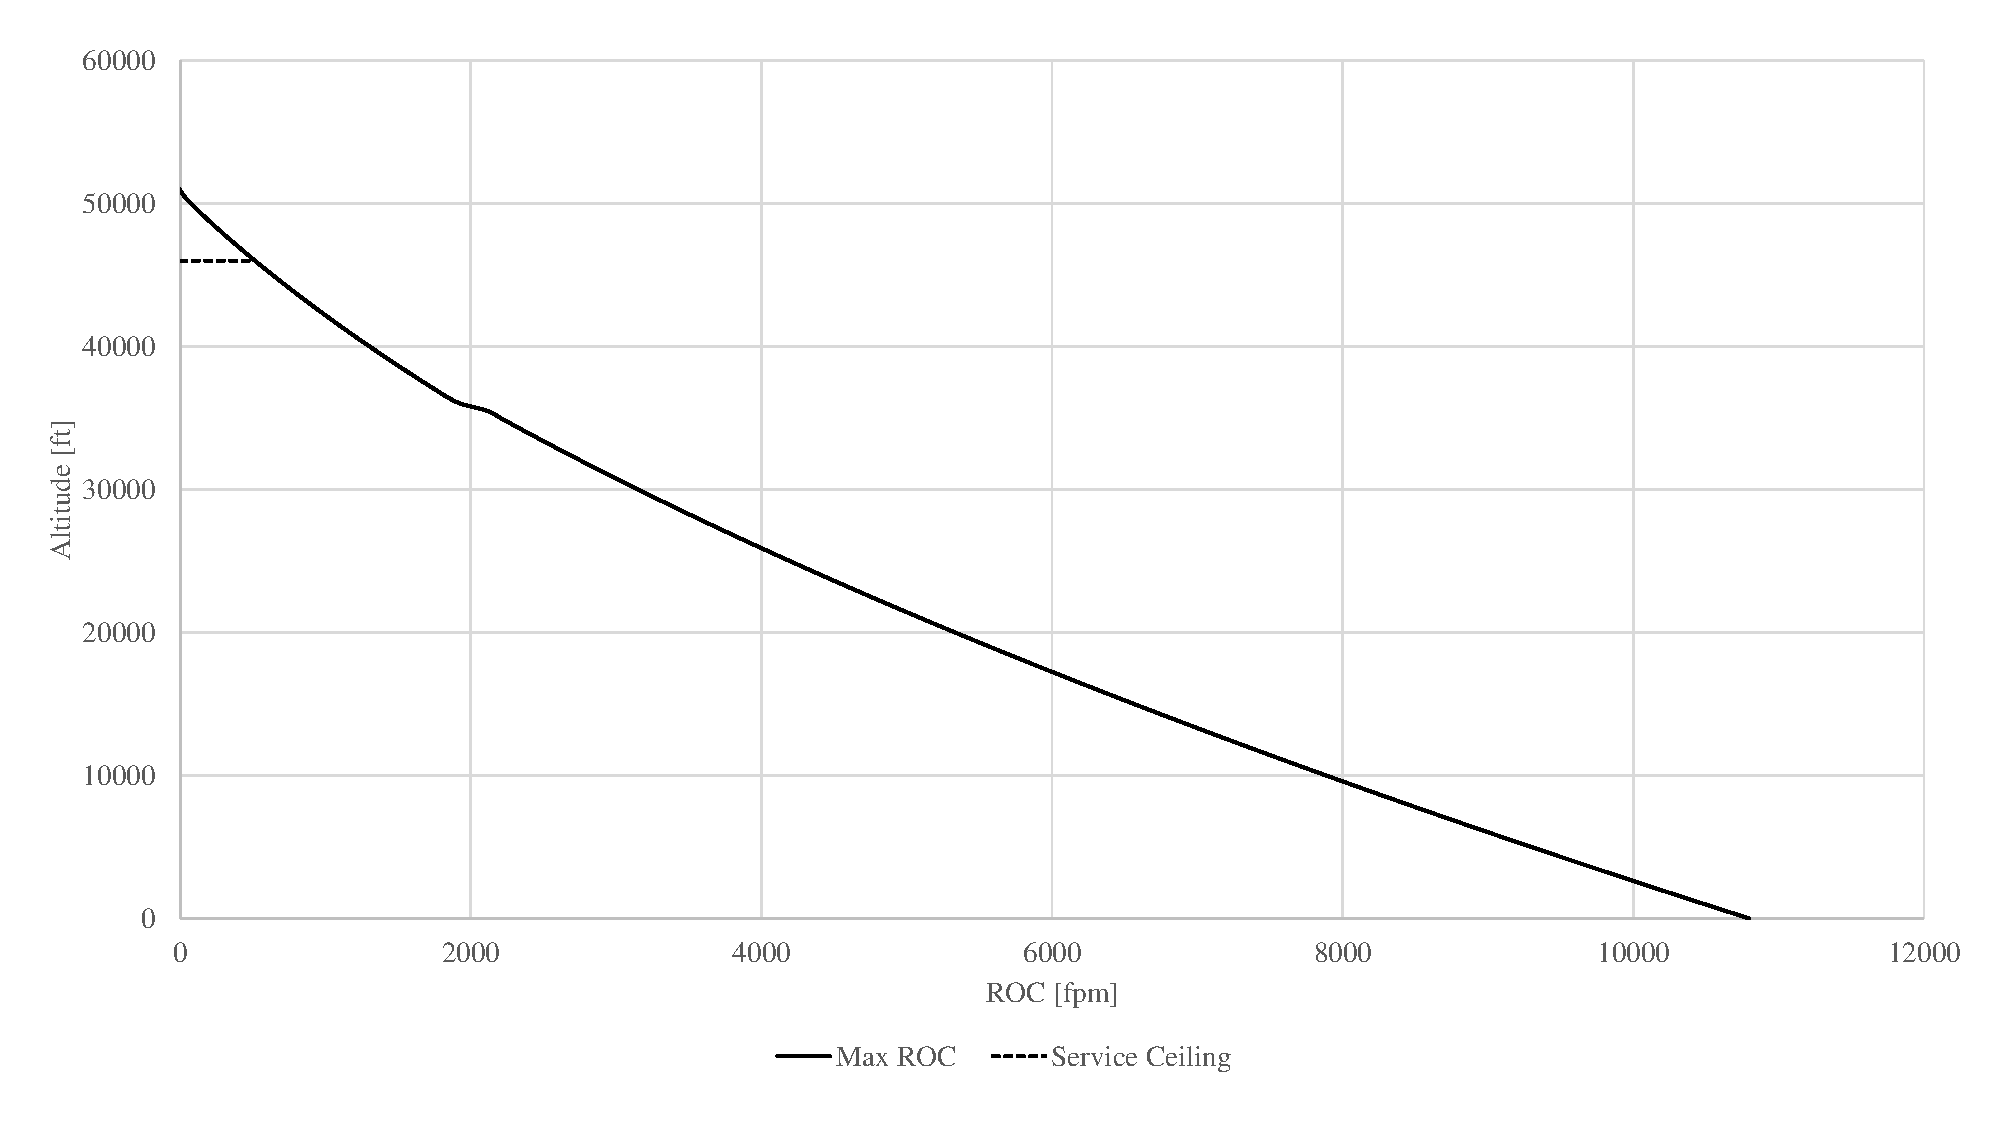
\includegraphics[width=1.0\textwidth]{Photos/Service_Ceiling.pdf}
    \caption{Service Ceiling -  SAM Mk 1}
    \label{serceil}
 \end{figure}

\subsection{Cruise (\textit{MK})}
An important part of the of the mission of the SAM Mk I is the cruise segment. In this segment, the design cruise speed was chosen to be M 0.775, as described in Section \ref{crusspeed}. Next, the aircraft will begin the cruise segment at an altitude of 37,000 ft, where it will step climb in segments of 2,000 ft to 39,000 ft and 41,000 ft, respectively. This process is performed to maintain a constant and high lift-to-drag ratio throughout the cruise segment of the design mission. Two methods were used to estimated the overall performance of the cruise segment. First, a time-step integration was used to determine the range and endurance of our aircraft. Each step climb was performed after a third of the allotted cruise fuel (which will be discussed in Section "Fuel per Mission Segment") was burned during the process. Once the allotted cruise fuel was all burned, the total range and total endurance of the aircraft was calculated. Second, the total range and total endurance were calculated using the Breguet-Range and Breguet-Endurance equations. This was then compared to the time-step integration method to determine the accuracy of both methods to one another. Table \ref{tab:cruise} shows the range, endurance, and percent error between both methods. 

\begin{table}[!h]
    \centering
    \caption{Cruise: Breguet Method and Time-step Integration}
    \begin{tabular}{|p{1in}||p{1in}|p{1.5in}|p{1in}|}\toprule 
     & \textbf{Breguet Method} & \textbf{Time-step Integration} & \textbf{\% Difference} \\ \hline \hline
    \textbf{Range [NM]} & 3,500 & 3,504 & 0.11 \\ \hline
    \textbf{Endurance [hr]} & 7.76 & 7.77 & 0.11 \\ 
    \bottomrule
    \end{tabular}
    \label{tab:cruise}
\end{table}

From the data, SAM Mk I successfully meets the range requirement set by the RFP. Additionally, it can be seen that the difference between the Breguet method and time-step integration is quite small, thus, solidifying the use of the Breguet method for cruise estimation. 

\subsection{Fuel per Mission Segment (\textit{MK})}
An important parameter to determine for SAM Mk I is how much fuel is required for the duration of the mission. The mission can be broken up into two main section: non-block and reserves. In the non-block section, the segments include Warm-up, Taxi, and TO (WUTTO), Climb, Cruise, Descend, 5 minute loiter at 5,000 ft, and Approach, Landing, and Taxi (ALT). The reserves will contain a climb to 30,000 ft, a 200 NM alternate to another airport, a 30 min loiter at the airport, descend, 5\% contingency fuel, and a 5 minute loiter at 5,000 ft. Weight fractions from Raymer\cite{raymer} were used for WUTTO and ALT. Fuel estimation for cruise and alternate destination was determined using Breguet range while the loiter segments used Breguet Endurance equations. Finally, all climb and descend values were estimated using a time-step integration method. Table \ref{fuelfrac} shows the calculated fuel fractions. 

\begin{table}[!h]
    \centering
    \caption{Fuel Fractions for Each Mission Segment}
    \begin{tabular}{|p{1.75in}||p{1in}|p{1.5in}|}\toprule 
    \textbf{Mission Segment} & \textbf{Fuel Weight [lb]} & \textbf{Calculated Fuel Fraction}\\ \hline \hline
    WUTTO & 6,750 & 0.985 \\ \hline
    Climb & 8,060 & 0.982  \\ \hline
    Cruise & 95,950 & 0.786 \\ \hline
    Descend & 6,420 & 0.986 \\ \hline
    ALT & 1,660 & 0.996 \\ \hline
    5 min Loiter (5,000 ft) & 910 & 0.997 \\ \hline
    Climb to 30,000 ft & 4,430 & 0.990 \\
    \hline
    200 NM Alternate & 2,090 & 0.995 \\ \hline
    30 min Loiter & 7,370 & 0.984 \\ \hline
    Descend & 5,160 & 0.988 \\ \hline
    5\% Contingency Fuel & 5,990 & 0.987 \\ \hline
    5 min Loiter (5,000 ft) & 1,240 & 0.997 \\ \hline
    \textbf{Total} & \textbf{146,860} & \textbf{0.679} \\
    \bottomrule
    \end{tabular}
    \label{fuelfrac}
\end{table}

\subsection{Drag per Mission Segment (\textit{MK})}
During each segment, there is associated parasitic drag and drag due to lift. Team Toucans utilized multiple methods for different segments of the mission. Specifically, the Climb, Cruise, and Descend segments were calculated using a time-step integration, while the Takeoff and Landing Segments utilized the drag equation. Additionally, the conditions for each of the segments were set by the RFP for takeoff and landing. Due to there being variations in the drag, Table \ref{dragseg} shows drag ranges for each segment of the mission. 

\begin{table}[h]
    \centering
    \caption{Drag per Mission Segment}
    \begin{tabular}{|p{1.5in}|p{1in}|}\toprule 
    \textbf{Mission Segment} & \textbf{Drag Range [lb]} \\ \hline \hline
    Takeoff & 0-46,000 \\ \hline
    Climb & 26,000-30,500   \\ \hline
    Cruise & 25,100-26,100 \\ \hline
    Descend & 20,500-27,400 \\ \hline
    Landing & 0-14,800 \\
    \bottomrule
    \end{tabular}
    \label{dragseg}
\end{table}

\subsection{Payload-Range Diagram (\textit{MK})}
The payload-range diagram is used to analyze the range of the aircraft as payload weight is traded for fuel weight. The payload-range diagram illustrating this relationship can be seen in Figure \ref{payrang}. The lines in the diagram were calculated using the Breguet-Range method. The top line up to point A uses a payload weight of 94,300 lb and a cruise fuel weight of 95,950 lb. Then, the line from point A to point B maximizes the total fuel capacity of SAM Mk 1, which adds about 44,140 lb of fuel to the cruise fuel weight and brings the total to 140,090 lb of cruise fuel weight. Finally, the line from point B to point C represents the aircraft going to zero payload weight at the same max fuel weight from the previous line. This results in the SAM Mk 1 having a maximum range of about 6,240 NM at zero payload weight and maximum fuel weight.

\begin{figure}[H]
    \centering
    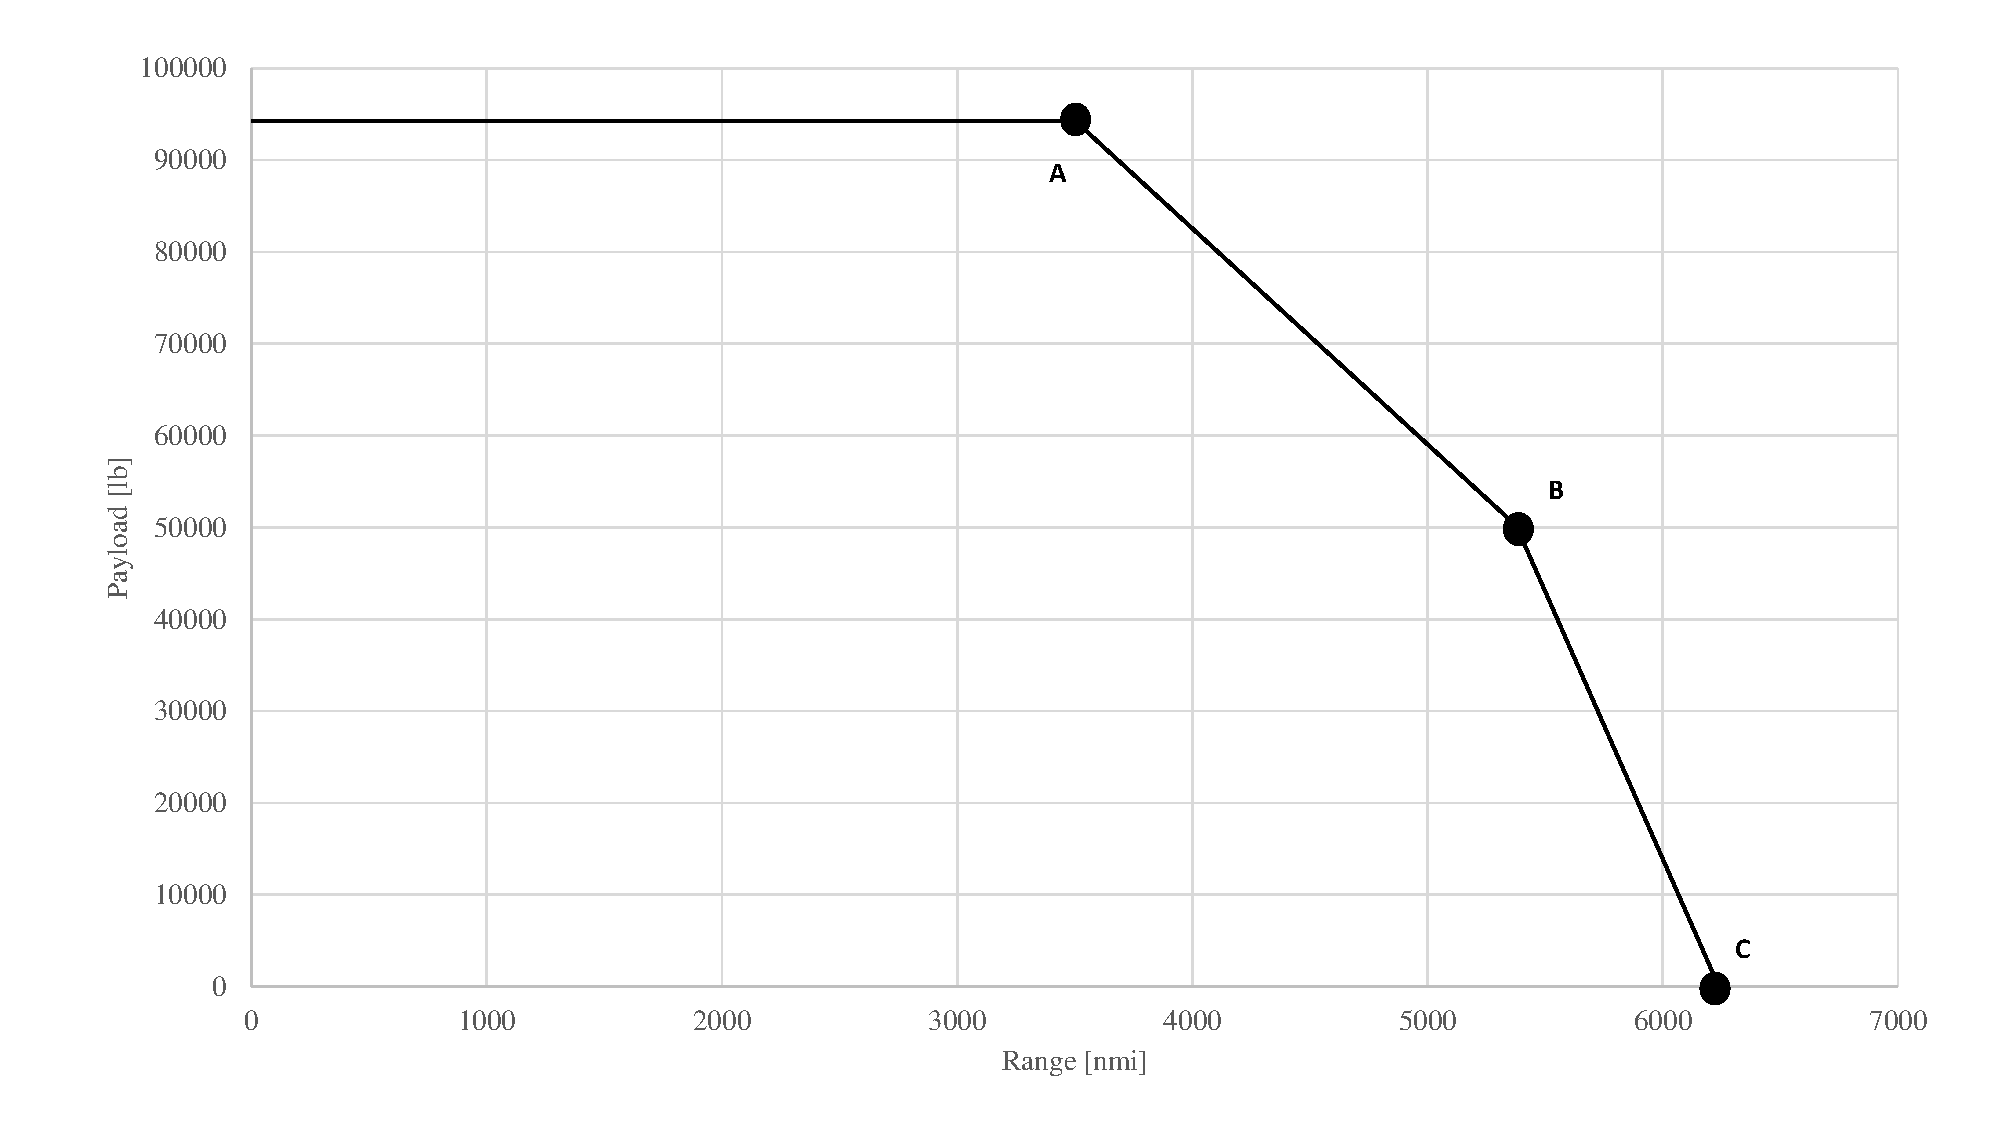
\includegraphics[width=1.0\textwidth]{Photos/Payload_Range.pdf}
    \caption{Payload-Range Diagram -  SAM Mk. I}
    \label{payrang}
 \end{figure}

\subsection{Flight Envelope (\textit{MK})}
\label{ssfl}
The flight envelope is an important diagram that demonstrates the capability of an aircraft, in terms of speed and what the altitude limits are. Additionally, it shows the service ceiling of the aircraft. For SAM Mk 1, the maximum and minimum design velocities at sea-level were determined to be 640 kts and 150 kts, respectively. The maximum velocity was determined from the max speed at which the aircraft could structurally fly (max dive speed), which will be discussed further in the Loads Section. The minimum speeds was bounded by the stall speed of the SAM Mk I. Furthermore, the absolute ceiling of SAM Mk I was determined to be 49,700 ft. This shows that SAM Mk I's cruising altitudes are within the minimum and maximum parameters. A visual representation of the flight envelope can be seen in Figure \ref{flyenv}, with the green shade corresponding to the velocity and altitude limits of the aircraft. 

\begin{figure}[!h]
    \centering
    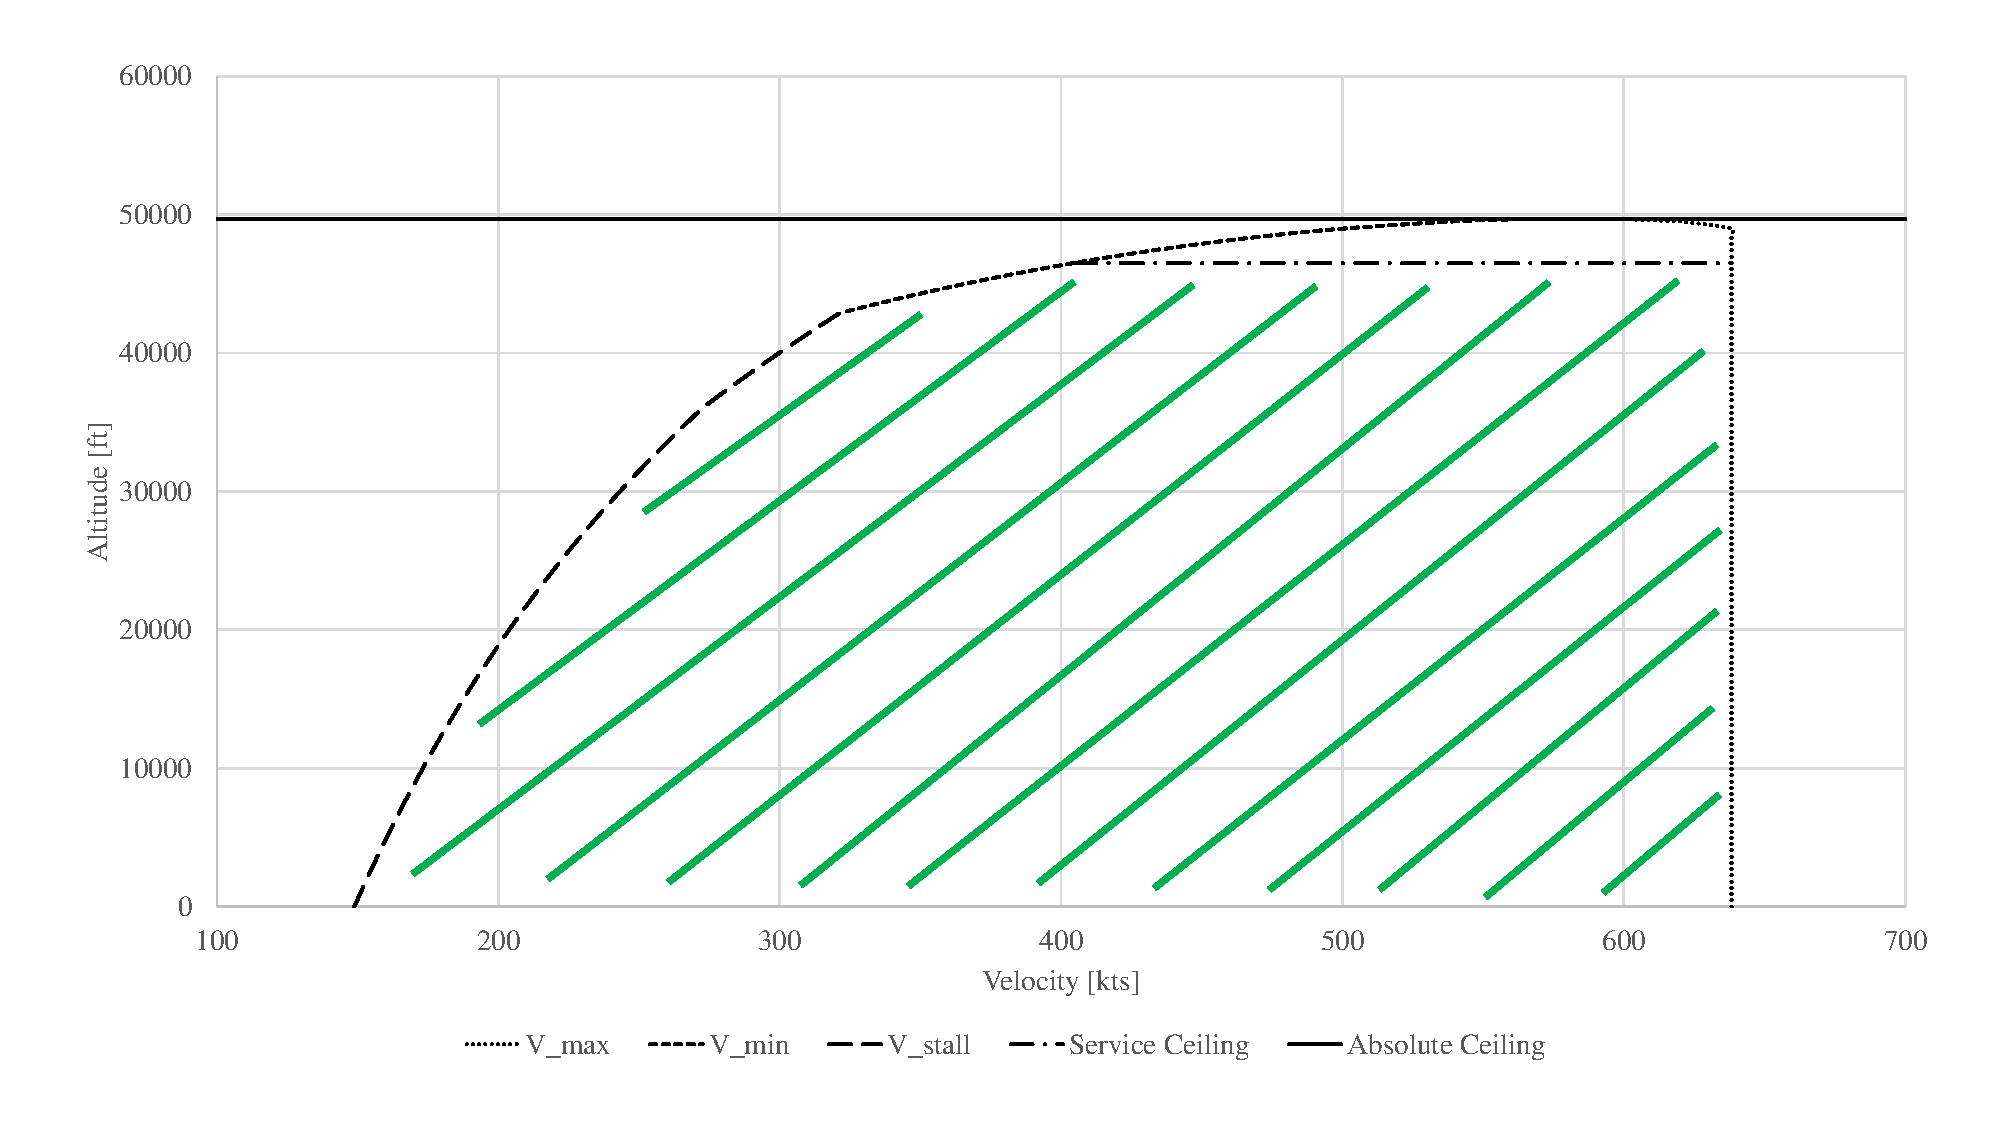
\includegraphics[width=1.0\textwidth]{Photos/Flight_Envelope.pdf}
    \caption{Flight Envelope (shaded) -  SAM Mk. I}
    \label{flyenv}
 \end{figure}
\clearpage

\subsection{Specific Excess Power Diagram (\textit{MK})}
One diagram that demonstrates the full capability of the aircraft is the Specific Excess Power, or $P_{s}$ diagram. This plot functions similarly to the flight envelope, as shown in Section \ref{ssfl}, but it does not reveal as much about the performance of the aircraft. The $P_{s}$ diagram is shown in Figure \ref{spexpw}, where specific excess power was calculated using the general specific excess power equation at varying Mach numbers and altitudes.

\begin{figure}[H]
    \centering
    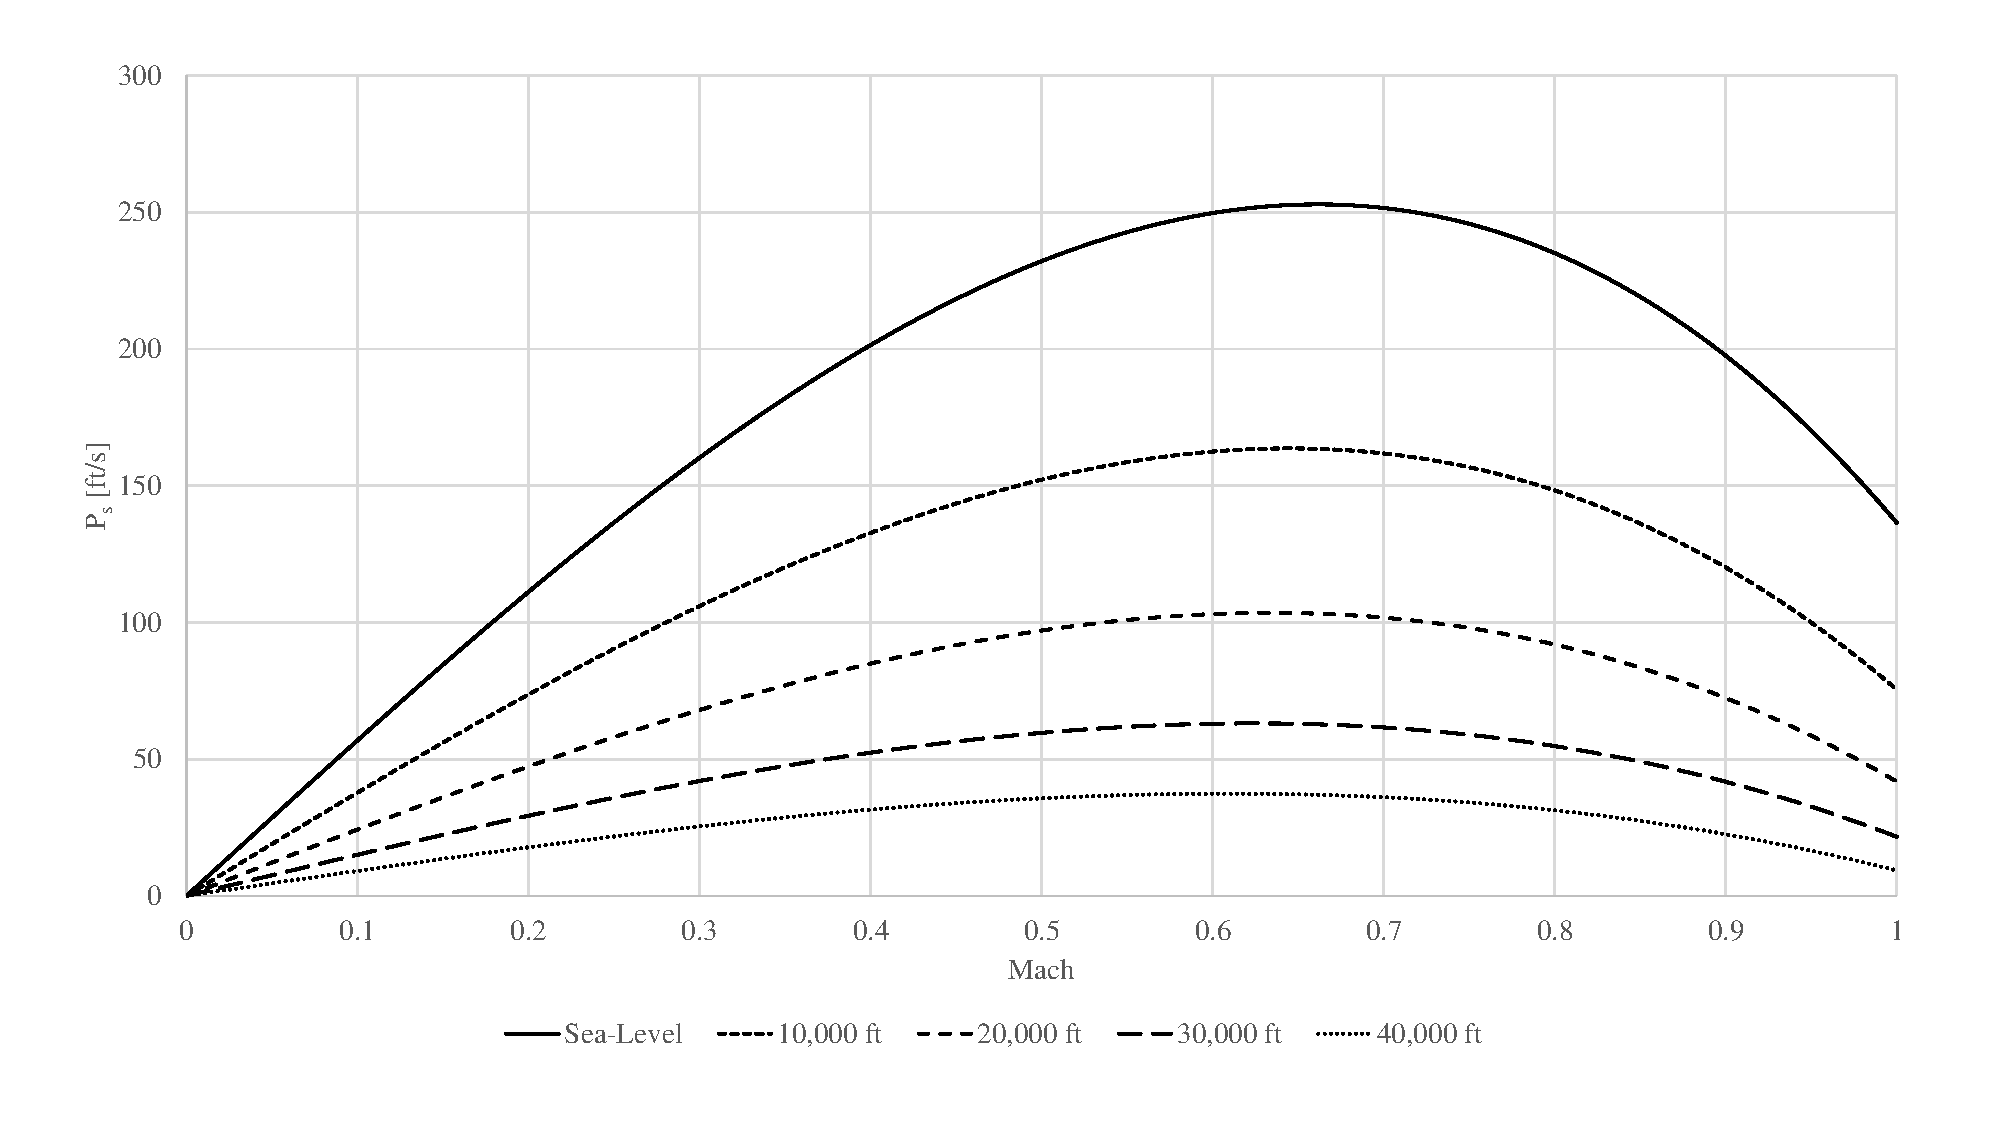
\includegraphics[width=1.0\textwidth]{Photos/Specific_Excess_Power.pdf}
    \caption{Specific Excess Power Diagram at Varying Speeds and Altitudes}
    \label{spexpw}
 \end{figure}
\clearpage

\subsection{Range-Mach Diagram}
A range-mach diagram can be used to determine the range of a particular aircraft with varying speeds while maintaining constant parameters, such as SFC, altitude, and L/D. Figure \ref{ramadg} displays this diagram at the cruising altitude of 37,000 ft. The Breguet Range equation was used to generate this plot, which follows a linear pattern. 

\begin{figure}[H]
    \centering
    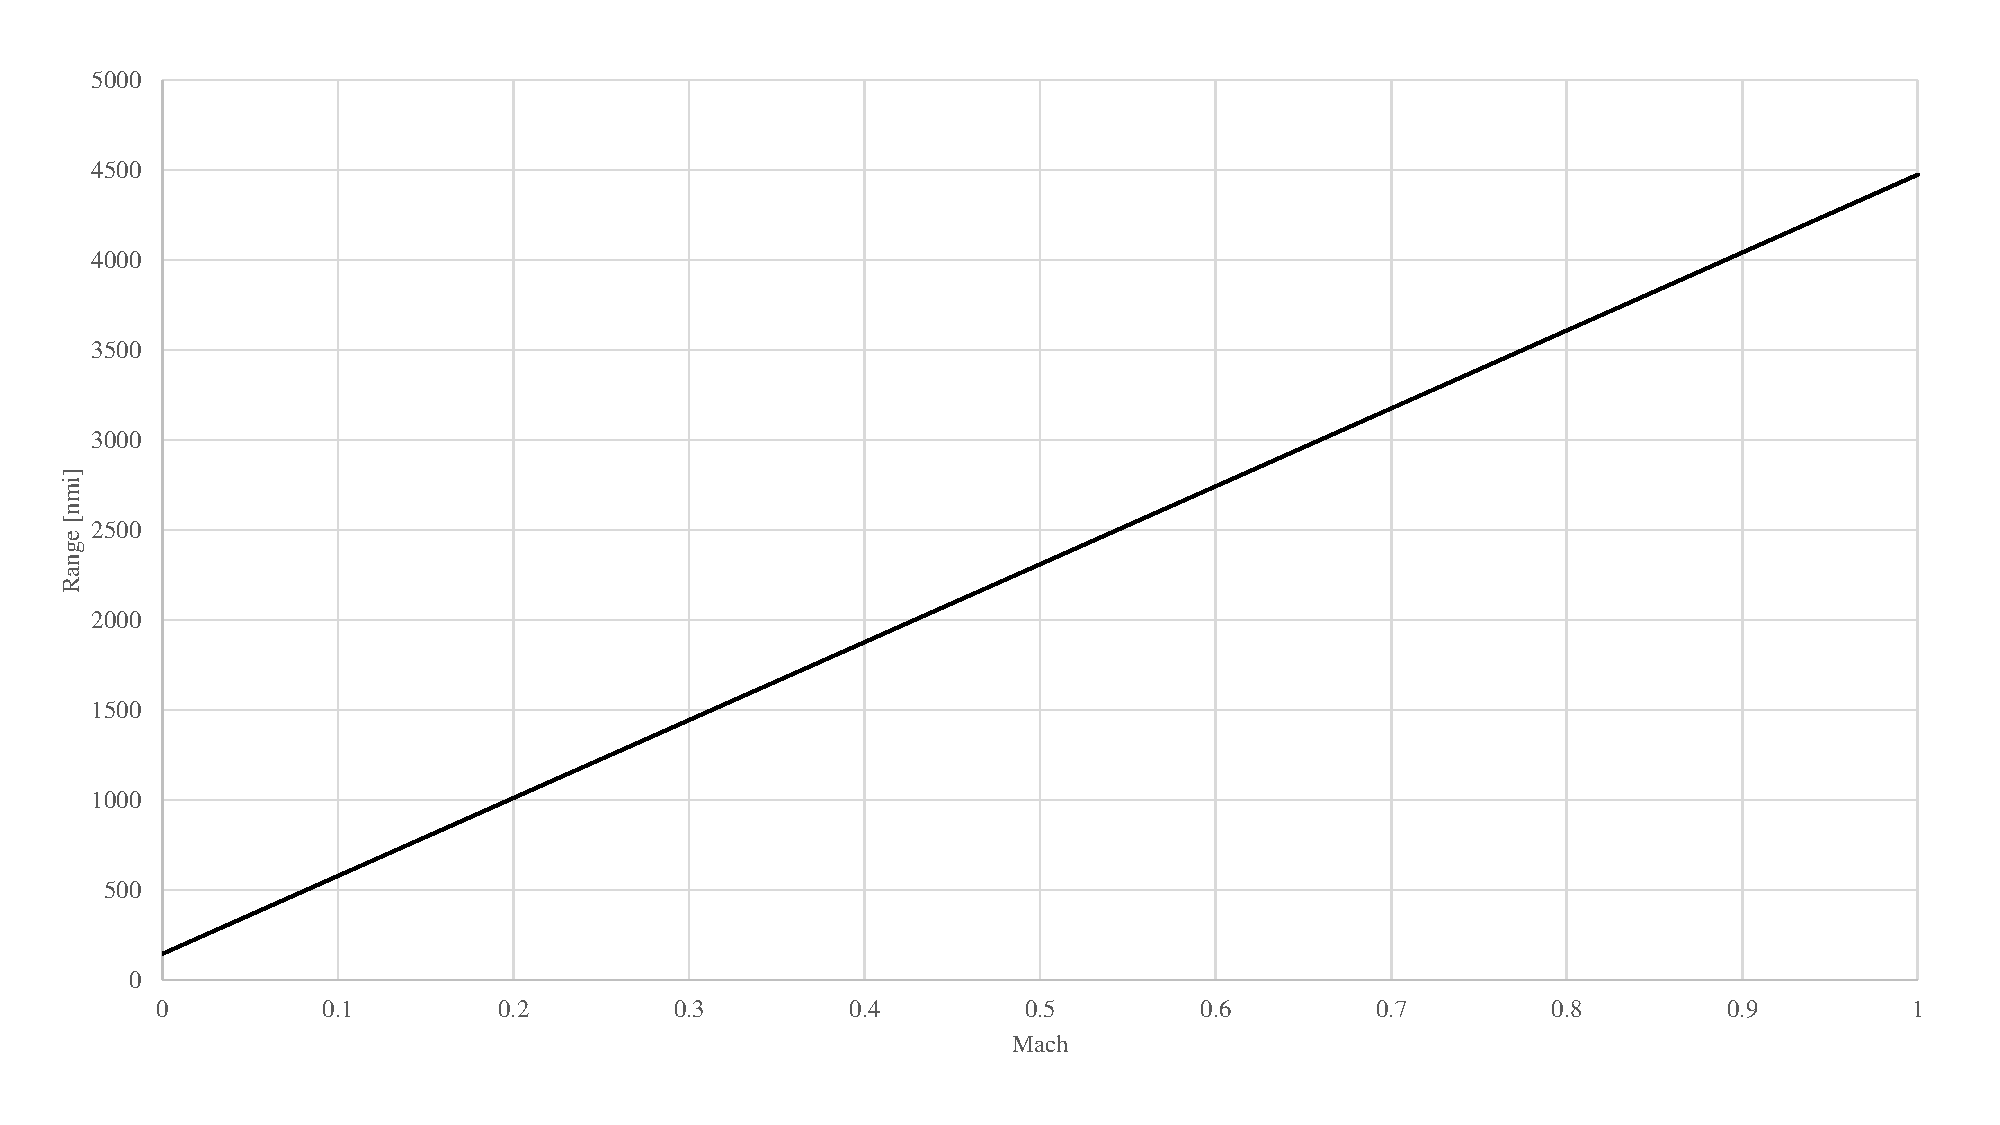
\includegraphics[width=1.0\textwidth]{Photos/Range_Mach.pdf}
    \caption{Range Mach Diagram @ 37,000 ft}
    \label{ramadg}
 \end{figure}

\subsection{Cruise and Loiter Performance Coefficients}
There are two main performance coefficients that are useful in determining the performance during loiter and cruise: $(\frac{C_{L}}{C_{D}})_{max}$ and $(\frac{C_{L}^{1/2}}{C_{D}})_{max}$. The coefficients correspond to the maximum endurance, or loiter, time and maximum range, or cruise, distance, respectively. By using the parabolic drag polar model, these coefficients become solely functions of the aircraft's geometry and $C_{D_{o}}$. Once these coefficients were obtained, the maximum endurance and range were calculated using the Breguet Endurance and Breguet Range equations, respectively. Table \ref{tab:loitcrui} displays the coefficient values as well as the maximum endurance and range. From Table \ref{tab:loitcrui}, our aircraft meets the requirements set forth by the RFP \cite{RFP}.

\begin{table}[!h]
    \centering
    \caption{Performance Coefficients with Max Endurance and Range}
    \begin{tabular}{|c|c|c|c|}\toprule 
    \boldmath{$(\frac{C_{L}}{C_{D}})_{max}$} & \boldmath{$(\frac{C_{L}^{1/2}}{C_{D}})_{max}$} & \textbf{Max Endurance [hr]} & \textbf{Max Range [NM]} \\ \hline \hline
    16.8 & 23.9 & 7.67 & 4,890 \\ 
    \bottomrule
    \end{tabular}
    \label{tab:loitcrui}
\end{table}

\clearpage
% MAT MAT MAT MAT MAT MAT MAT MAT MAT I THINK IM LIKE 97% done with THE TAKE OFF CD POSSIBLY MAYBE AT LEAST EARLY CALCULATION
% This so far without wing: 0.00098708 but I'm adding this to the wing analysis in XFLR.  O yaeh we probably can get away with assumptions and then blame the stupid aero guy for being incapable of finding these coefficients T.T
%  I WOULD NEVER BLAME YA!
% AWESOME! idk if ill have time ot include it in this report but after pdr i will for sure update the sheet


% \textcolor{red}{
% \begin{itemize}
%     \item Discuss performance analysis for takeoff and landing (accounting for ground roll and obstacle clearance), rate of climb, cruise, loiter, and service ceiling.
%     \begin{itemize}
%         \item Account for alternate conditions specified in RFP (grass, altitude, etc.) and CFR 23.67 (i.e. single engine-out takeoff)
%     \end{itemize}
% \item AIAA
% \subitem A description of the design missions defined for the proposed concepts for use in
% calculations of mission performance as per design objectives. This includes the
% selection of cruise altitude(s) and cruise speed/cruise Mach supported by pertinent
% trade analyses and discussion
% \subitem Aircraft performance summaries shall be documented and the aircraft flight envelope
% shall be shown graphically.
% \subitem Payload range chart(s)
% \subitem A V-n diagram for the aircraft with identification of necessary aircraft velocities and design load factors \hl{Or Loads disc. W/ Chris}
% \item All else per Merret --> SEE COMPASS
% \item \hl{Important aerodynamic characteristics and aerodynamic performance for key mission segments and requirements AERO or PERF}
% \end{itemize}}